
\begin{figure}[hp]
% 
\subcaptionbox{\label{fig:cluster6-Aa}}
{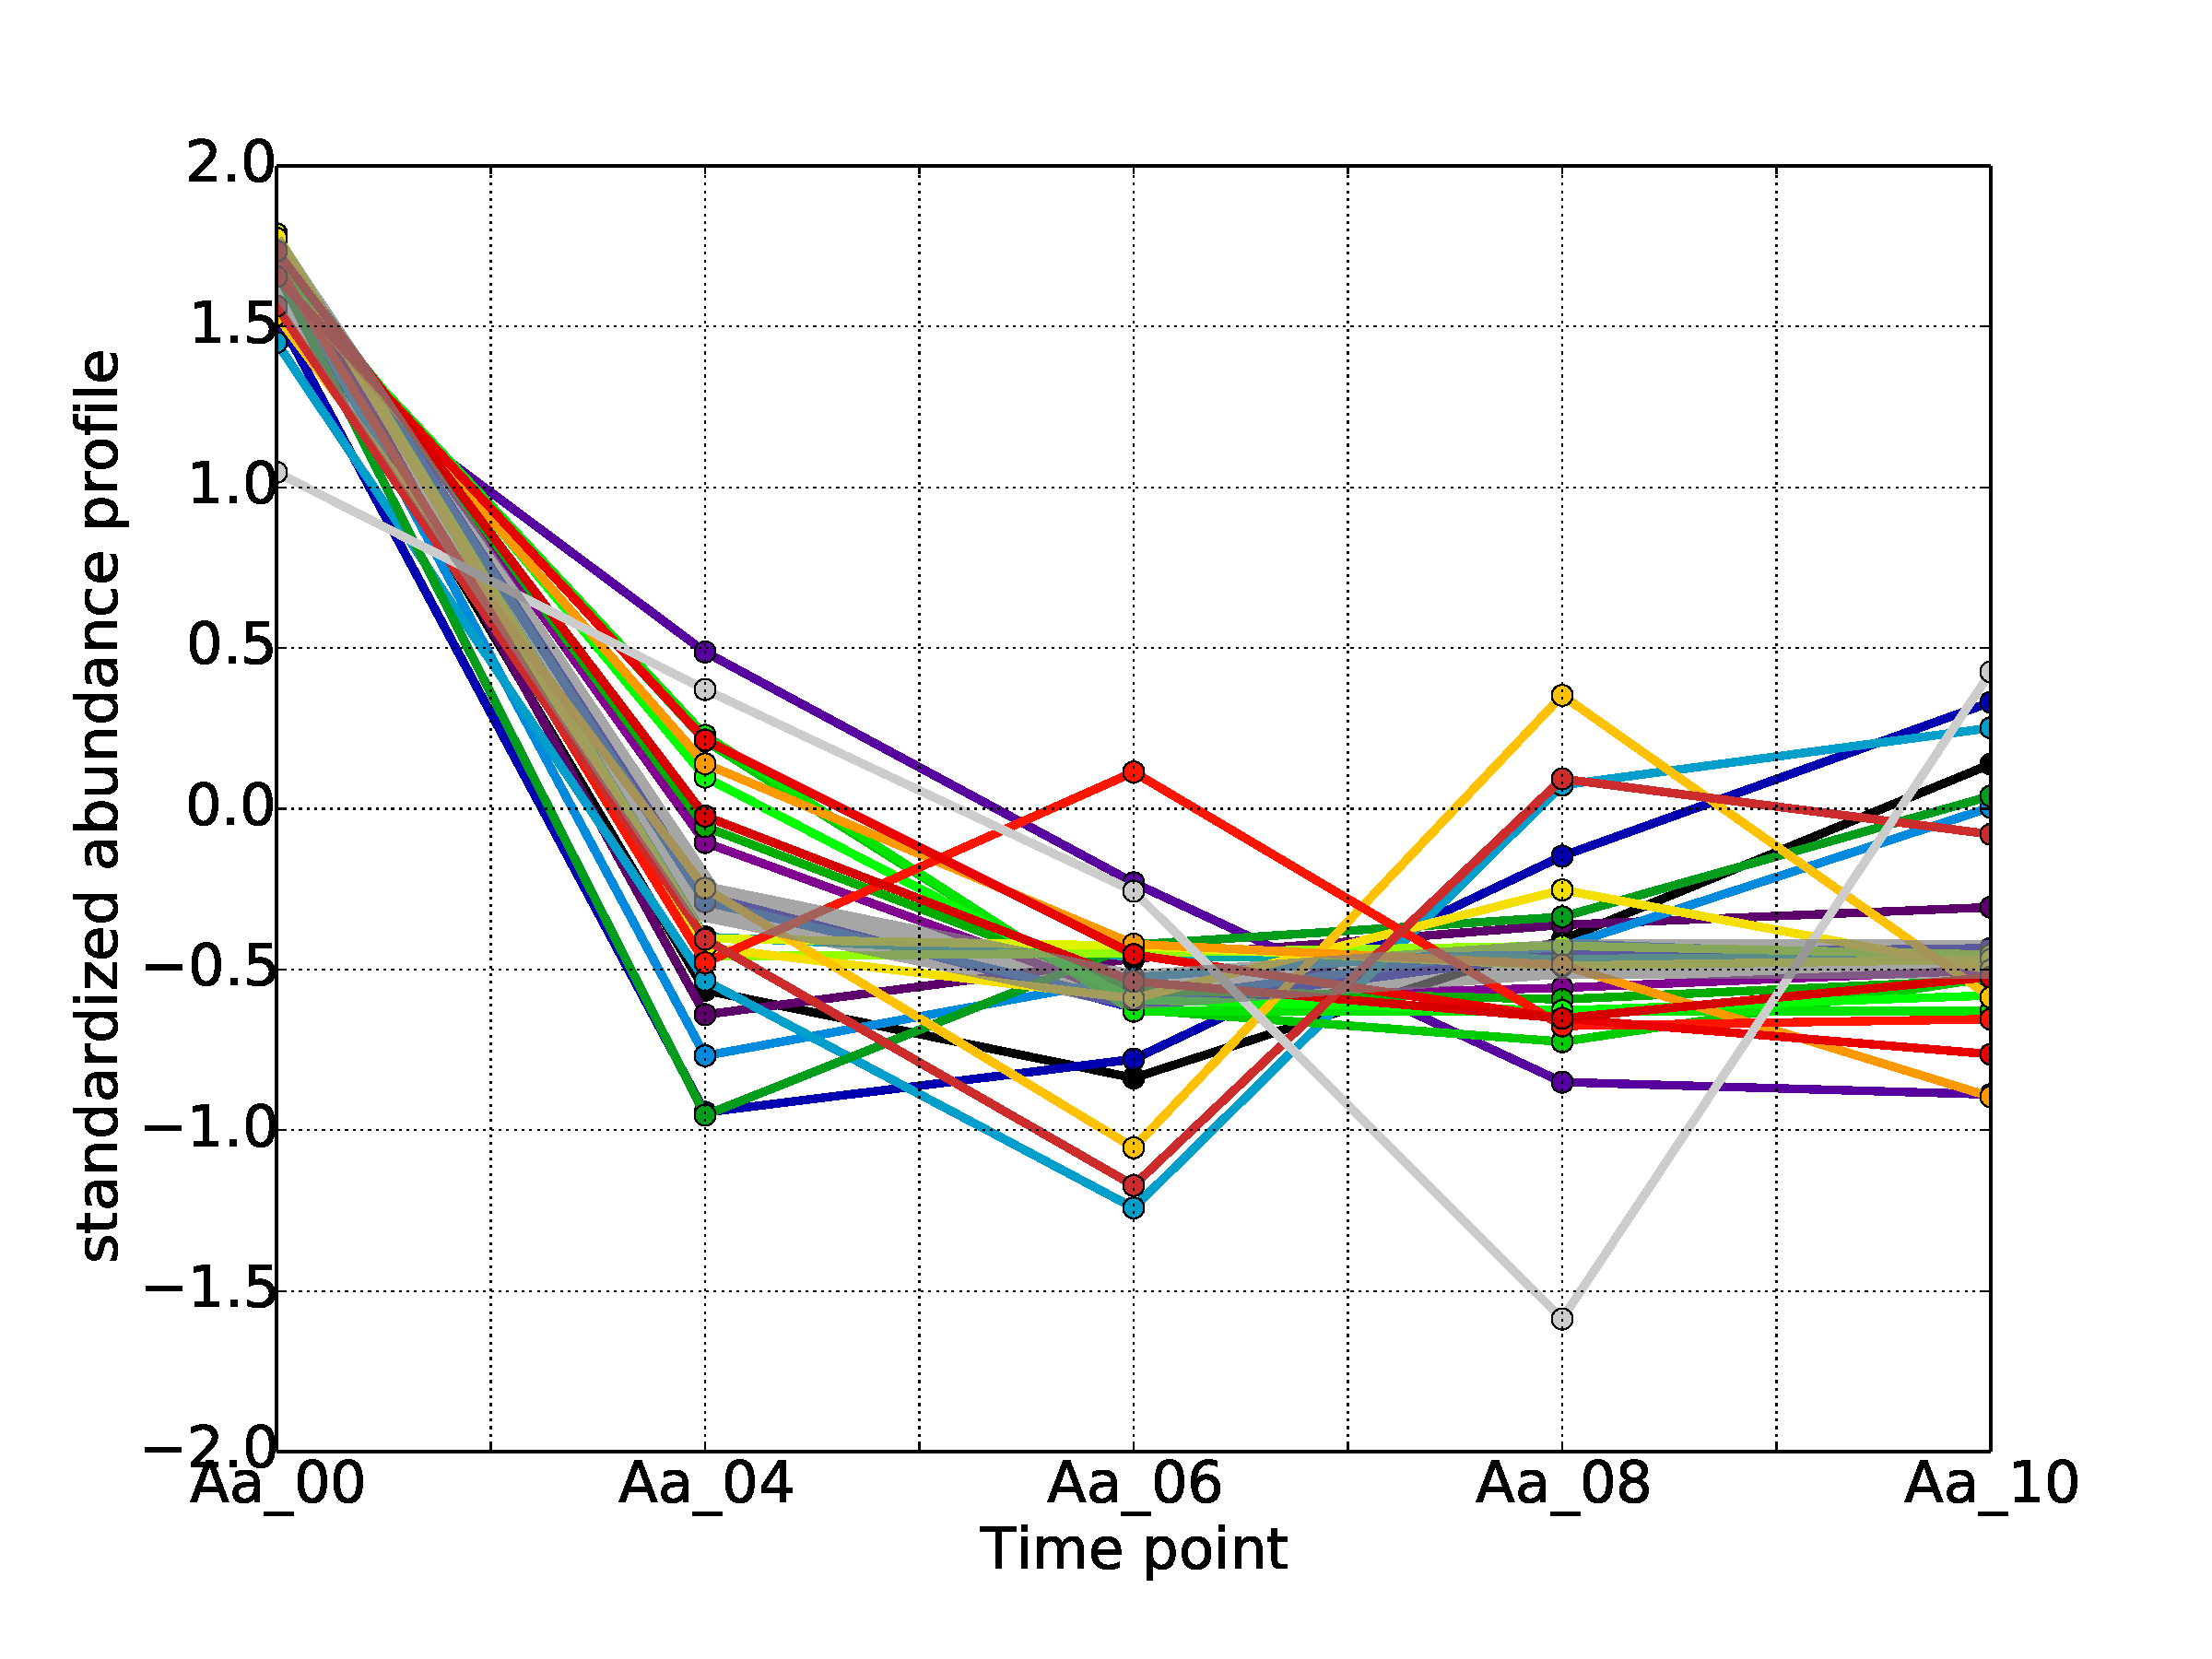
\includegraphics[width=.5\linewidth]{figures/figs/ecr_and_insects_ptci_20130918_orthodb7/downAfter4_gene_profiles_from_cummerbund/Aa_downAfter4_cls6_Ag_target_FPKMs_vb_orthos.pdf}}
%
\subcaptionbox{\label{fig:cluster6-Ag}}
{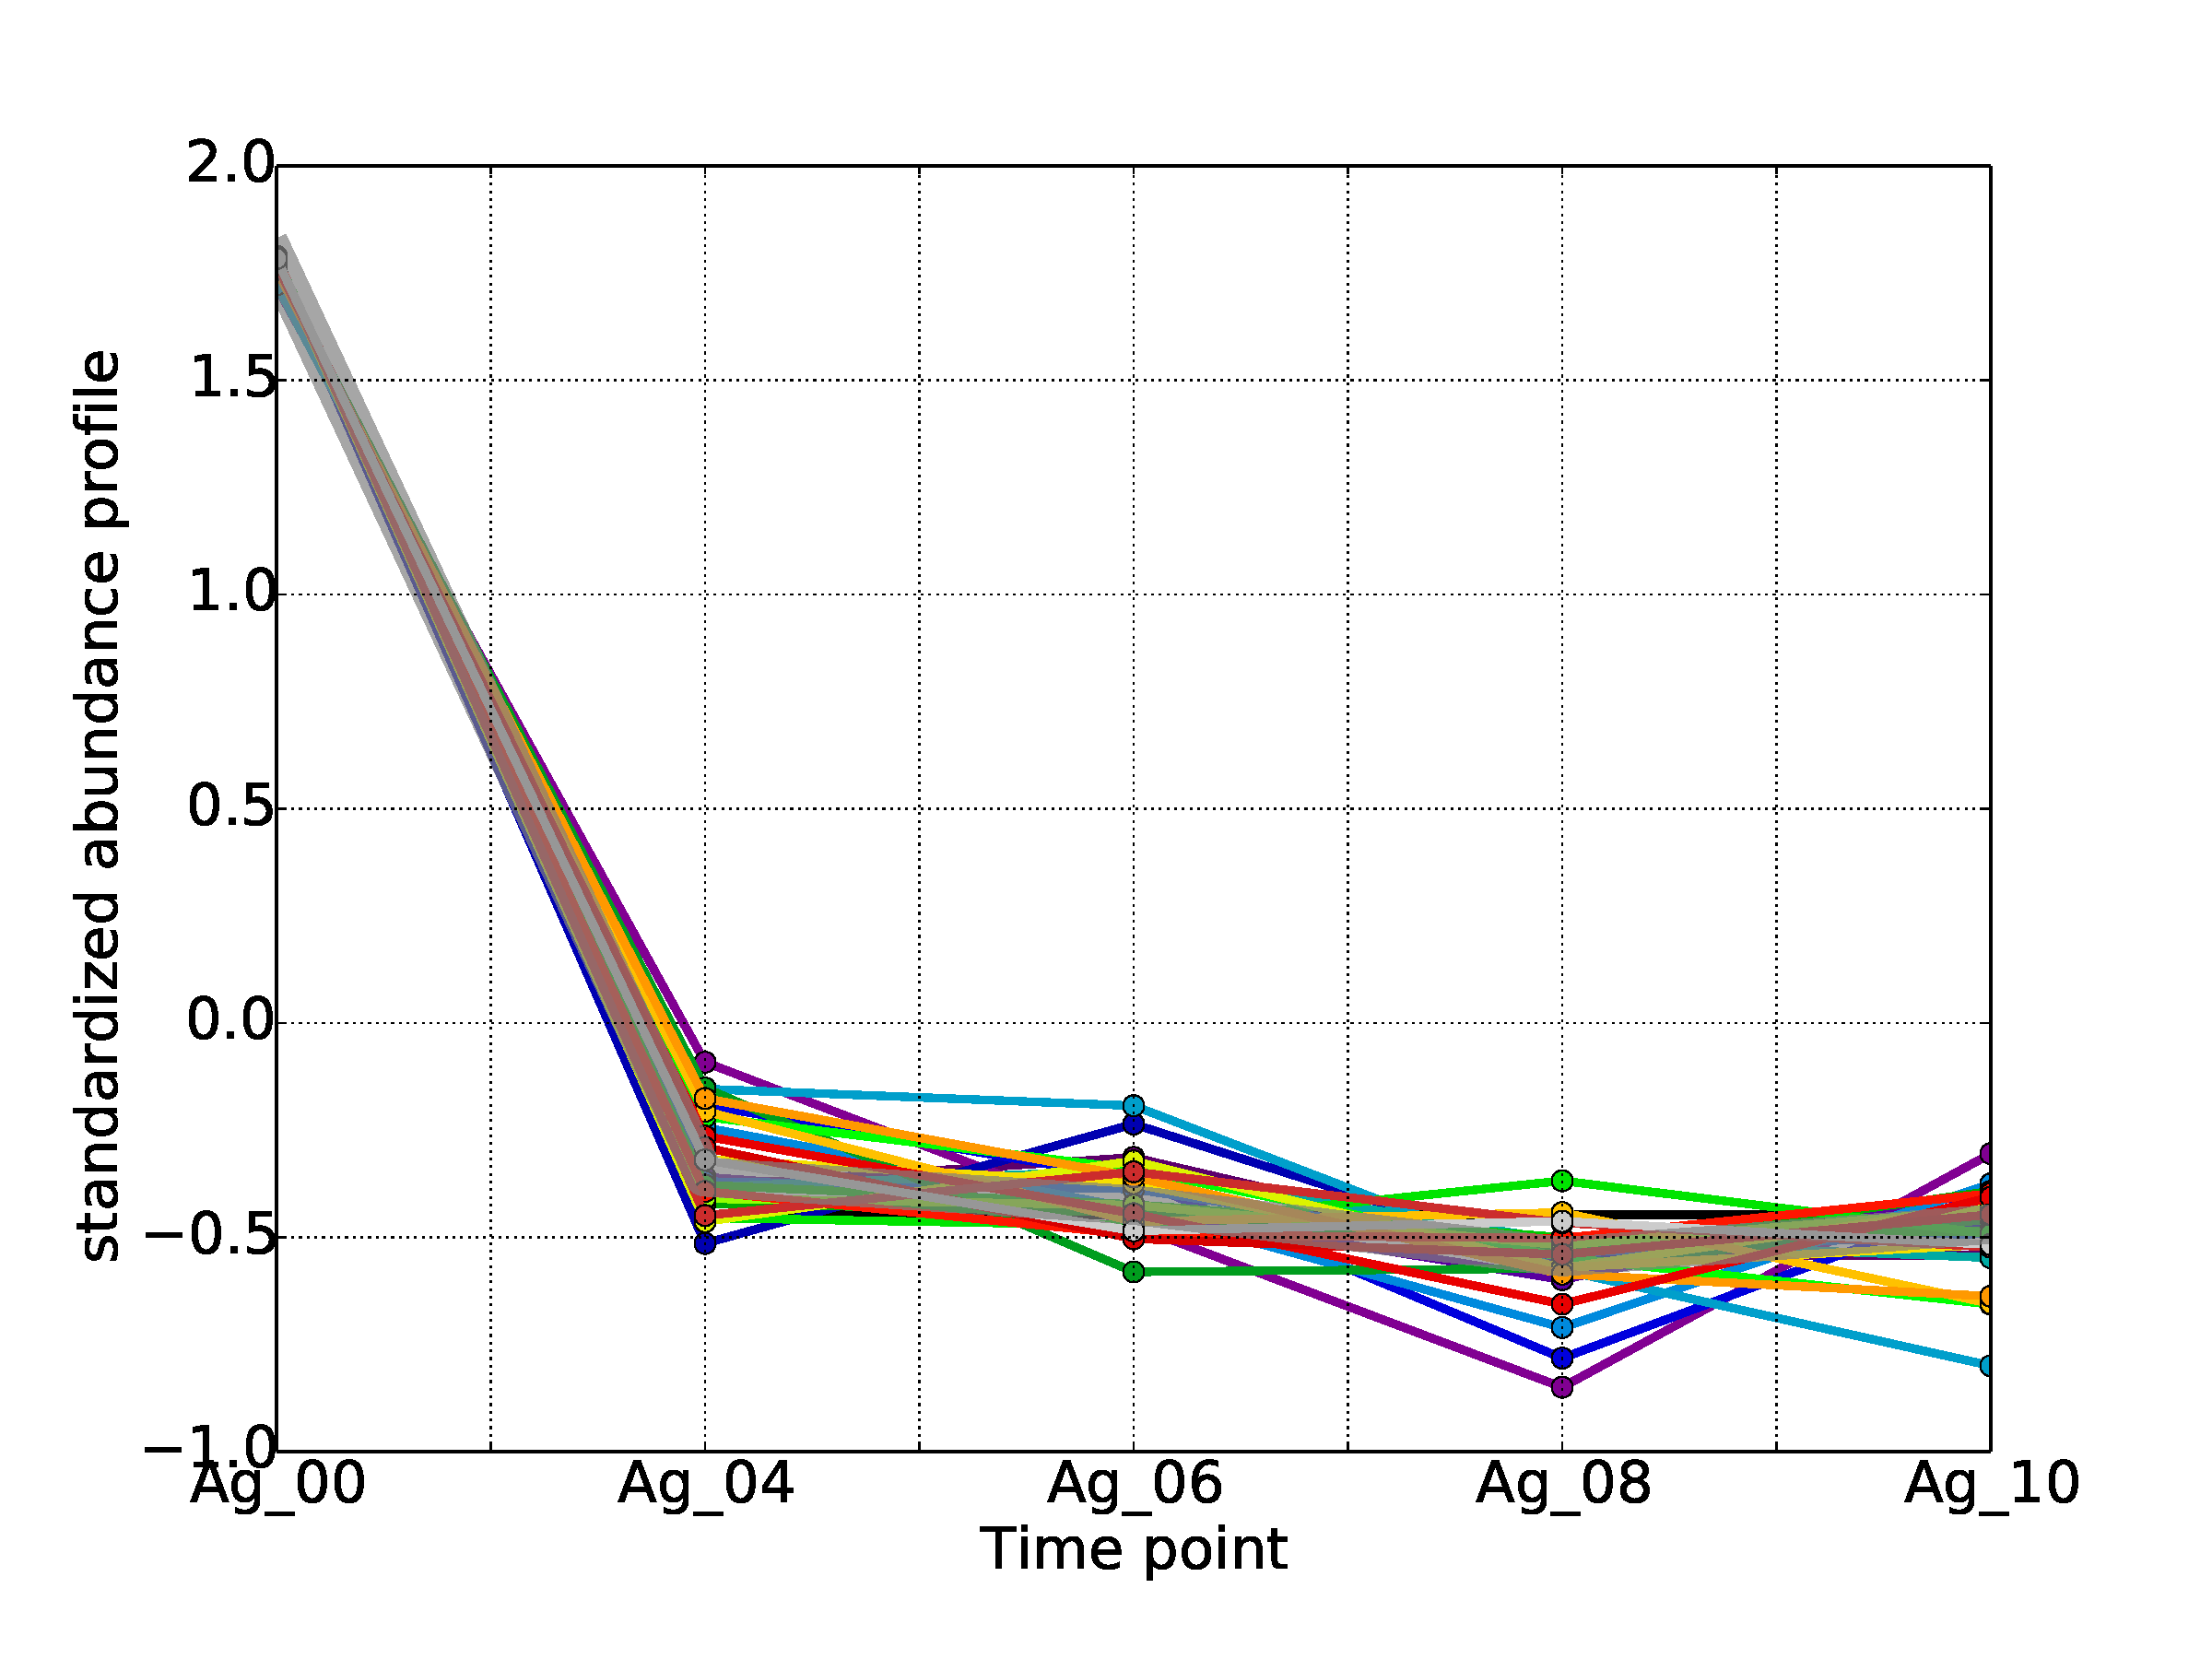
\includegraphics[width=.5\linewidth]{figures/figs/ecr_and_insects_ptci_20130918_orthodb7/downAfter4_gene_profiles_from_cummerbund/Ag_downAfter4_cls6_Ag_target_FPKMs_vb_orthos.pdf}}
%
\subcaptionbox{\label{fig:cluster6-Cq}}
{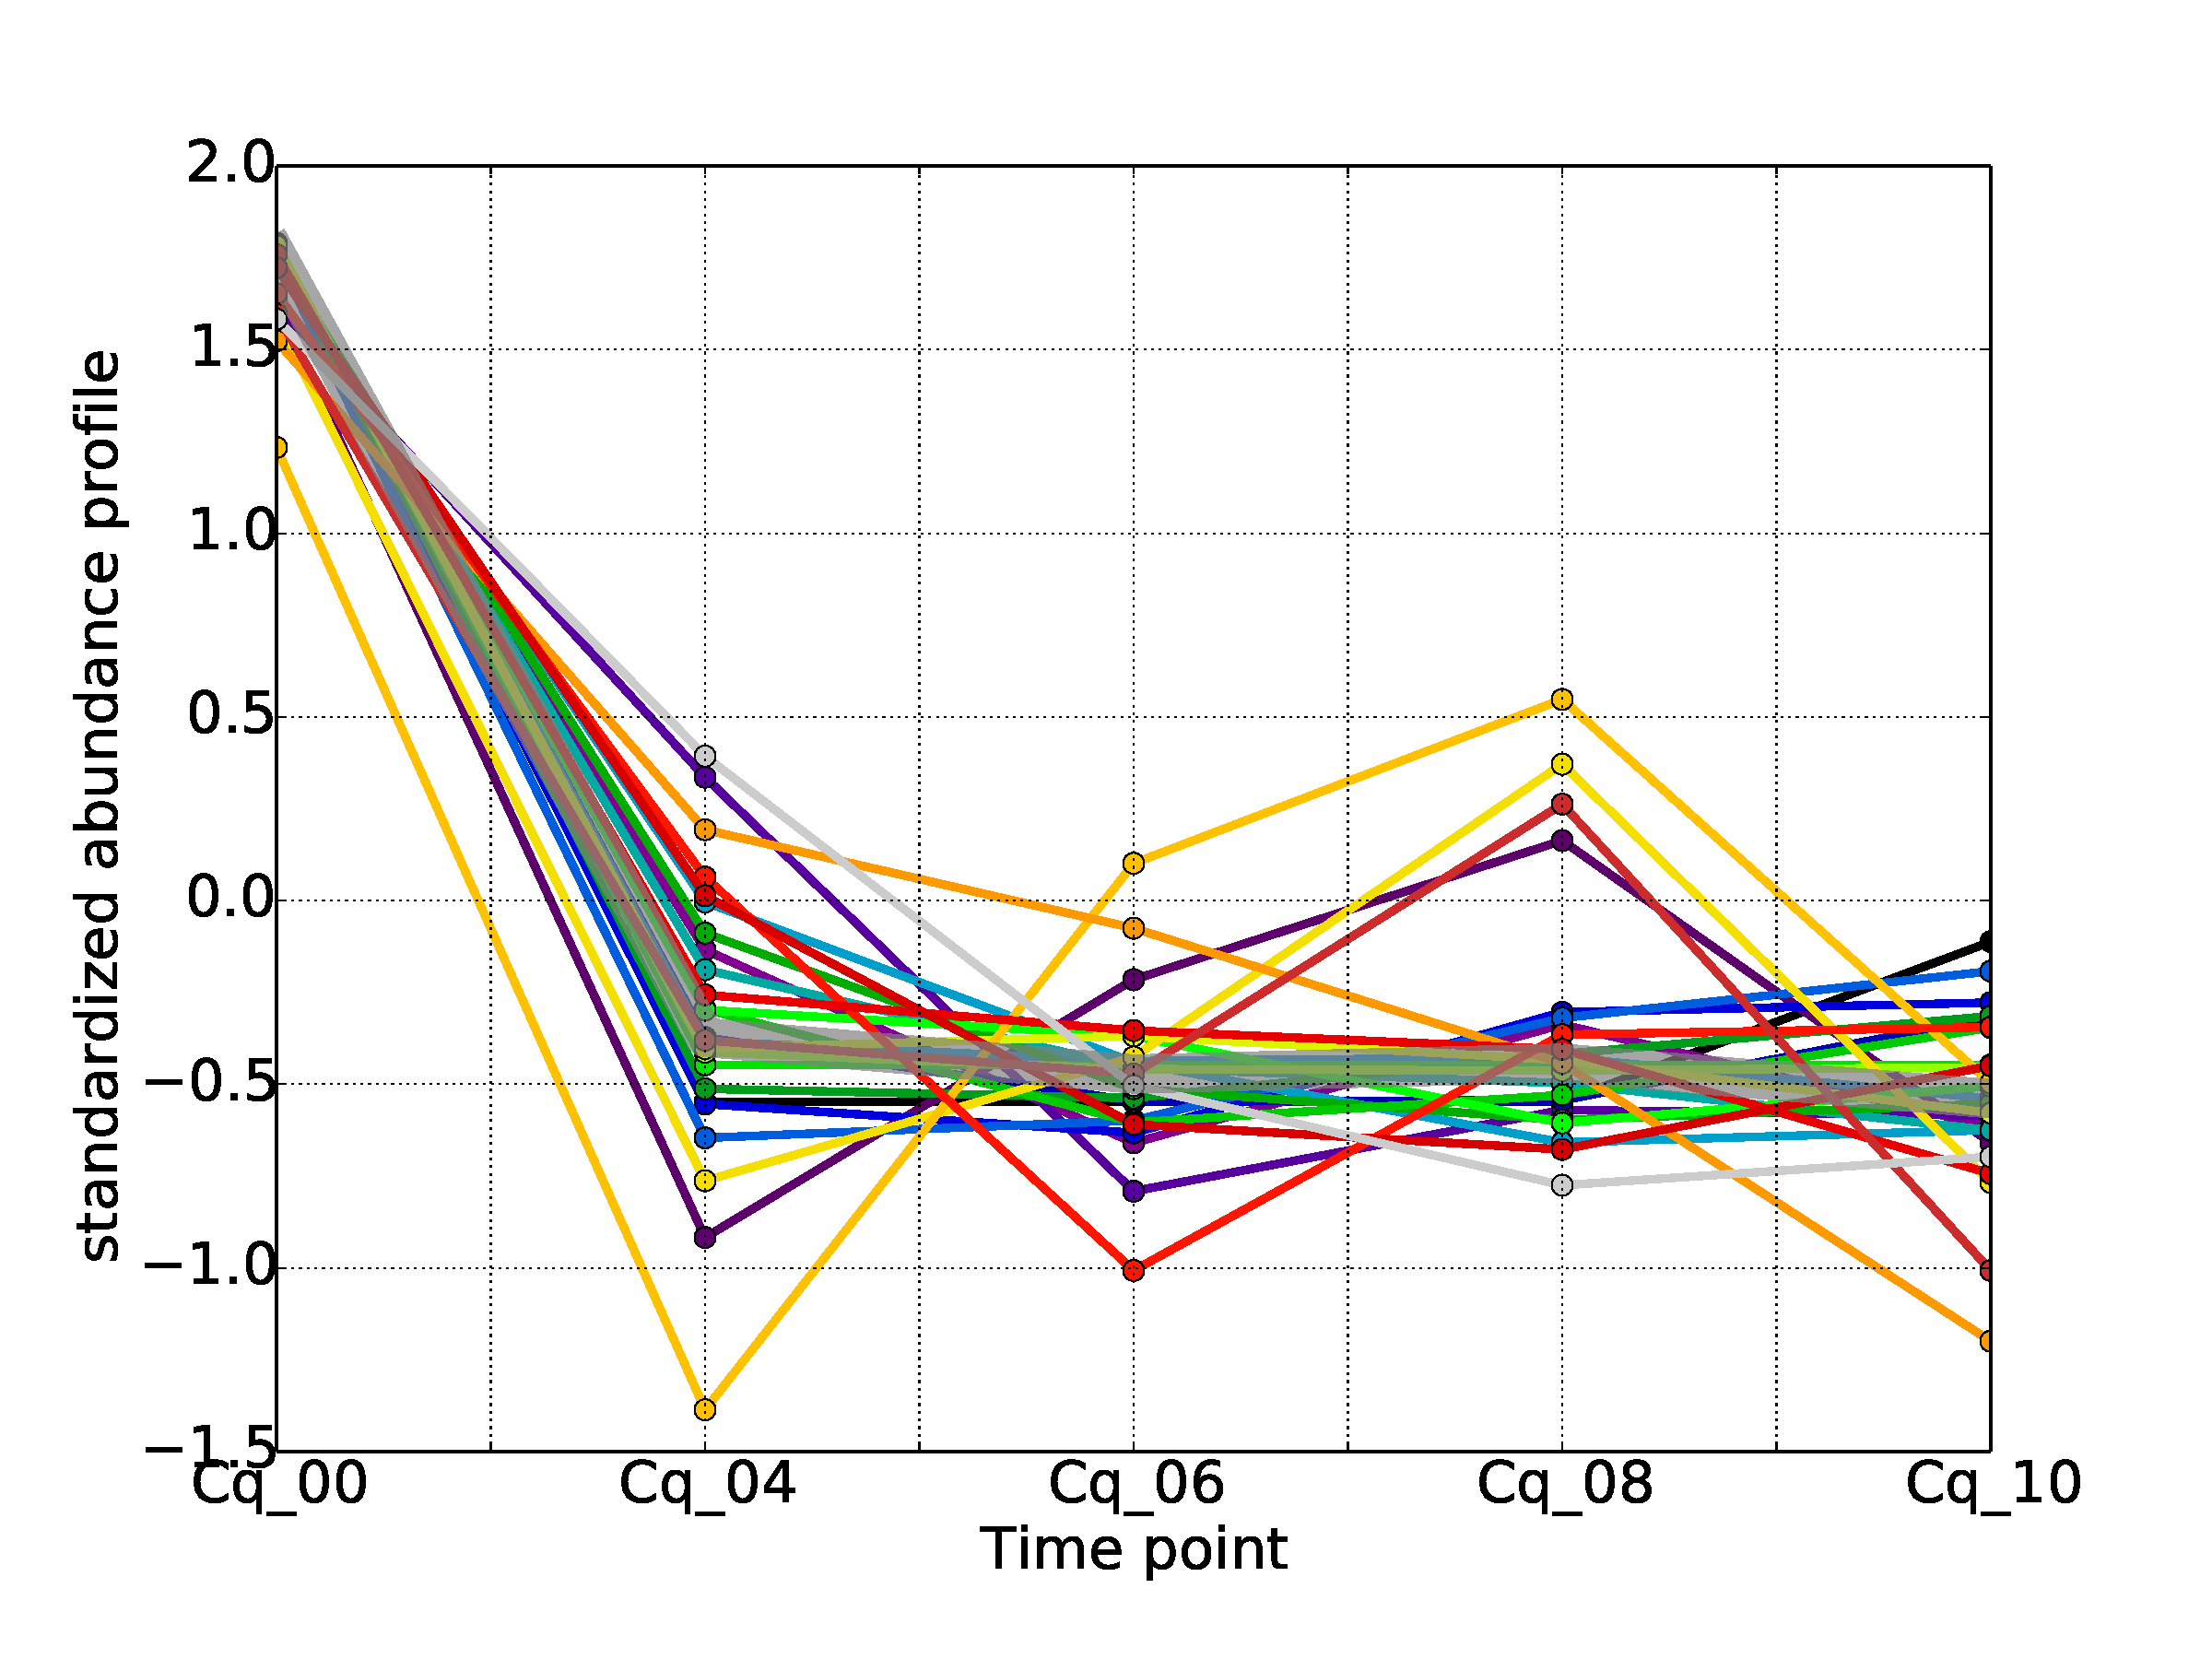
\includegraphics[width=.5\linewidth]{figures/figs/ecr_and_insects_ptci_20130918_orthodb7/downAfter4_gene_profiles_from_cummerbund/Cq_downAfter4_cls6_Ag_target_FPKMs_vb_orthos.pdf}}
% 
\caption[Orthologs of cluster 6]{\sf \textbf{Orthologs of cluster 6 (down after 4h):}\\
The same color scheme is used for each species which means that orthologs are given the same color in all three panels.
The thick, transparent gray line represents the median \gls{mAP} for the panel.
\textbf{(A)} \Aa.
\textbf{(B)} \Ag.
\textbf{(C)} \Cq.
}\label{fig:cluster6}
\end{figure}